\section{Random Variables}
\subsection{Random variables}
\begin{bdef}{Random variables}\label{randomvariables}
    When an experiment is performed, we are often more interested in a function of the outcome as opposed to the actual outcome itself. For instance, when tossing a handful of dice, we may care more about the sum of the numbers rolled than the separate values of each die, or when flipping coins, we may care more about the total number of heads flipped than the actual sequence of flips.

    These quantities of interest -- more formally, these functions from $S$ to $\Real$ -- are known as \textbf{random variables}. Because the value of a random variable is determined by the outcome of the experiment, we may assign probabilities to the possible values of the random variable.
\end{bdef}
\begin{changebar}
    \begin{example}
        Suppose our experiment consists of tossing 3 fair coins. If we let $Y$ denote the number of heads that appear, then $Y$ is a random variable with range $\left\{ 0, 1, 2, 3 \right\}$ and respective probabilities \[
            \begin{aligned}
                P\left\{ Y = 0 \right\} &= P(\left\{ (T, T, T) \right\}) &= \frac{1}{8} \\
                P\left\{ Y = 1 \right\} &= P(\left\{ (H, T, T), (T, H, T), (T, T, H) \right\}) &= \frac{3}{8} \\
                P\left\{ Y = 2 \right\} &= P(\left\{ (H, H, T), (H, T, H), (T, H, H) \right\}) &= \frac{3}{8} \\
                P\left\{ Y = 3 \right\} &= P(\left\{ (H, H, H) \right\}) &= \frac{1}{8}
            \end{aligned}    
        \]
        We also have \[
            1 = P\left( \bigcup^3_{i = 0} \left\{ Y = i \right\} \right) = \sum^3_{i = 0} P\left\{ Y = i \right\}    
        \]
    \end{example}
\end{changebar}

\begin{changebar}
    \begin{example}
        Four balls are to be randomly selected, without replacement, from an urn that contains 20 balls numbered 1 through 20. If $X$ is the largest ball selected, then $X$ is a random variable that takes on one of the values $4, 5, \dots, 20$. Because each of the $\displaystyle \binom{20}{4}$ possible selections of $4$ of the $20$ balls is equally likely, the probability that $X$ takes on each of its possible values is \[
            P\left\{ X = i \right\}\frac{\binom{i - 1}{3}}{\binom{20}{4}},\: i = 4, \dots, 20.    
        \] This is because the number of selections that result in $X = i$ is the number of selections that result in the ball numbered $i$ and three of the balls numbered $1$ through $i - 3$ being selected. As there are $\displaystyle \binom{1}{1}\binom{i - 1}{3}$ such selections, the preceding follows.
    \end{example}
\end{changebar}

\begin{changebar}
    \begin{example}
        Independent trials consisting of the flipping of a coin having probability $p$ of coming up heads are continually performed until either a head occurs or a total of $n$ flips is made. If we let $X$ denote the number of times the coin is flipped, then $X$ is a random variable taking on one of the values $1, 2, 3, \dots, n$, with respective probabilities \[
            \begin{aligned}
                P\left\{ X = 1 \right\} &= P\left\{ (h) \right\} &=& p \\
                P\left\{ X = 2 \right\} &= P\left\{ (t, h) \right\} &=& (1-p)p \\
                P\left\{ X = 3 \right\} &= P\left\{ (t, t, h) \right\} &=& (1-p)^2p \\
                \vdots && \vdots & \\
                P\left\{ X = n - 1 \right\} &= P\left\{ (\underbrace{t, t, \dots, t}_{n - 2}, h) \right\} &=& (1-p)^{n-2}p \\
                P\left\{ X = n \right\} &= P\left\{ (\underbrace{t, t, \dots, t}_{n - 1}, t), (\underbrace{t, t, \dots, t}_{n - 1}, h) \right\} &=& (1-p)^{n-1}
            \end{aligned}    
        \]
    \end{example}    
\end{changebar}
\begin{bdef}{Distribution function}\label{distributionfunction}
    For a random variable $X$, the function $F: \Real \to [0, 1]$ defined by \[
        F(x) = P\left\{ X \leq x \right\}
    \] is called the \textbf{cumulative distribution function}, or more simply, the \textbf{distribution function} of $X$. Thus, the distribution function specifies, for all real values $x$, the probability that the random variable is less than or equal to $x$.
    
    Suppose that $a \leq b$. Then, because the event $\left\{ X \leq a \right\}$ is contained in the event $\left\{ X \leq b \right\}$, it follows that $F(a) \leq F(b)$. In other words, $F(x)$ is a nondecreasing function of $x$. Other properties of $F$ are given in \autoref{cumdistproperties}.
\end{bdef}
\pagebreak
\subsection{Discrete random variables}
\begin{bdef}{Discrete random variables}\label{discreterandomvariables}
    A random variable that can take on at most a countable number of possible values is said to be \textbf{discrete}.
\end{bdef}
\begin{bdef}{Probability mass function}\label{probabilitymassfunction}
    For a discrete random variable $X$, we define the \textbf{probability mass function} $p(a)$ of $X$ by \[
        p(a) = P\left\{ X = a \right\}.    
    \] $p(a)$ is positive for at most a countable number of values of $a$. That is, if $X$ must assume one of the values $x_1, x_2, \dots, x_n$, then \[
        \begin{cases}
            p(x_i) \geq 0 & \text{for } i = 1, 2, \dots \\
            p(x) = 0 & \text{otherwise} 
        \end{cases}    
    \] Since $X$ must take one of the values $x_i$, we have \[
        \sum^\infty_{i = 1} p(x_i) = 1.    
    \]
\end{bdef}
It is often instructive to plot the probability mass function by plotting $x_i$ on the $x$-axis against $p(x_i)$ on the $y$-axis. For example, the graph of the probability mass function of the random variable representing the sum of two dice would look like:
\begin{center}    
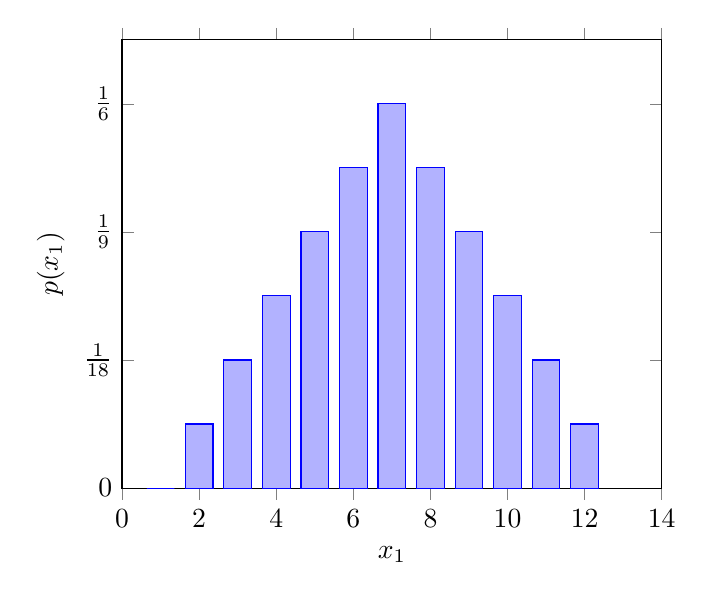
\begin{tikzpicture}
    \begin{axis}[
        ybar, 
        xmin = 0, 
        xmax = 14, 
        ymin = 0, 
        ymax = 7/36,
        yticklabel style={/pgf/number format/frac, /pgf/number format/frac shift=2}, 
        ytick={0, 2/36, 4/36, 6/36},
        xlabel={$x_1$}, 
        ylabel={$p(x_1)$}]
        \addplot coordinates {
            (1, 0)
            (2, 1/36)
            (3, 2/36)
            (4, 3/36)
            (5, 4/36)
            (6, 5/36)
            (7, 6/36)
            (8, 5/36)
            (9, 4/36)
            (10, 3/36)
            (11, 2/36)
            (12, 1/36)
        };
    \end{axis} 
\end{tikzpicture}
\end{center}
\begin{changebar}
    \begin{example}
        The probability mass function of a random variable $X$ is given by $p(i) = c\lambda^i/i!$, $i = 0, 1, \dots,$ where $\lambda$ is some positive value. Find \begin{enumerate}[label=(\alph*)]
            \item $P\left\{ X = 0 \right\}$.
            \item $P\left\{ X > 2 \right\}$.
        \end{enumerate}
    \end{example}
    \begin{solution}
        Since $\displaystyle \sum^\infty_{i = 0} p(i) = 1$, we have \[
            c \sum^\infty_{i = 0} \frac{\lambda^i}{i!} = 1.    
        \] Because $\displaystyle e^x = \sum^\infty_{i = 0} \frac{x^i}{i!}$, this implies that \[
            ce^\lambda = 1 \text{ or } c = e^{-\lambda}.    
        \]
        Thus, we have: \begin{enumerate}[label=(\alph*)]
            \item $P\left\{ X = 0 \right\} = p(0) = e^{-\lambda}\lambda^0/0! = e^{-\lambda}$
            \item \[
                \begin{aligned}
                    P\left\{ X > 2 \right\} &= 1 - P\left\{ X \leq 2 \right\} \\
                    &= 1 - P\left\{ X = 0 \right\} - P\left\{ X = 1 \right\} - P\left\{ X = 2 \right\} \\
                    &= 1 - e^{-\lambda} - \lambda e^{-\lambda} - \frac{\lambda^2e^{-\lambda}}{2}.
                \end{aligned}    
            \]
        \end{enumerate}
    \end{solution}
\end{changebar}

We can see that the distribution function $F$ can be expressed in terms of $p(a)$ by \[
    F(a) = \sum_{\text{all $x \leq a$}} p(x).    
\] If $X$ is a discrete random variable whose possible values are $x_1, x_2, x_3, \dots$, where $x_1 < x_2 < x_3 < \dots$, then $F$ is a step function; that is, the value of $F$ is constant in the intervals $(x_{i-1}, x_i)$, then takes a step (or jump) of size $p(x_i)$ at $x_i$. For example, if $X$ has a probability mass function given by \[
    p(1) = \frac{1}{4},\, p(2) = \frac{1}{2},\, p(3) = \frac{1}{8},\, p(4) = \frac{1}{8},
\] then its cumulative distribution function is \[
    \begin{cases}
        0 & a < 1 \\
        \frac{1}{4} & 1 \leq a < 2 \\
        \frac{3}{4} & 2 \leq a < 3 \\
        \frac{7}{8} & 3 \leq a < 4 \\
        1 & 4 \leq a
    \end{cases}
\]
\pagebreak
\subsection{Expected value}
\begin{bdef}{Expected value}\label{expectedvalue}
    If $X$ is a discrete random variable having a probability mass function $p(x)$, then the \textbf{expectation}, or \textbf{expected value}, of $X$, denoted $E\left[ X \right]$, is defined by \[
        E\left[ X \right] = \sum_{x:\, p(x) > 0} xp(x).    
    \] In other words, the expected value of $X$ is a weighted average of the possible values that $X$ can assume, weighted by the probability that $X$ assumes it.
\end{bdef}
This definition of expectation is partly motivated by the frequency interpretation of probabilities. This assumes that if an infinite sequence of independent replications of an experiment is performed, then, for any event $E$, the proportion of time that $E$ occurs will be $P(E)$. Consider a random variable $X$ that must taken on one of the values $x_1, x_2, \dots, x_n$, with respective probabilities $p(x_1), p(x_2), \dots, p(x_n)$, and think of $X$ as representing our winnings in a single game of chance. That is, with probability $p(x_i)$, we shall win $x_i$ units. By the frequency interpretation, if we play this game continually, then the proportion of time that we win $x_i$ will be $p(x_i)$. Since this is true for all $i$, $i = 1, 2, \dots, n$, it follows that our average winnings per game will be \[
    \sum^n_{i = 1} x_ip(x_i) = E\left[ X \right].
\]
\begin{changebar}
    \begin{example}\label{dieexpected}
        Find $E\left[ X \right]$, where $X$ is the outcome when we roll a fair die.
    \end{example}
    \begin{solution}
        Since $p(1) = p(2) = p(3) = p(4) = p(5) = p(6) = \frac{1}{6}$, we obtain \[
            E\left[ X \right] = 1\left( \frac{1}{6} \right) + 2\left( \frac{1}{6} \right) + 3\left( \frac{1}{6} \right) + 4\left( \frac{1}{6} \right) + 5\left( \frac{1}{6} \right) + 6\left( \frac{1}{6} \right) = \frac{7}{2}.    
        \]
    \end{solution}
\end{changebar}
\begin{changebar}
    \begin{example}
        A contestant on a quiz show is presented with two questions, questions 1 and 2, which he is to attempt to answer in some order he chooses. If he decides to try question $i$ first, then he will be allowed to go on to question $j$, $j \neq i$, only if his answer to question $i$ is correct. If his initial answer is incorrect, he is not allowed to answer the other question. The question is to receive $V_i$ if he answers question $i$ correctly, $i = 1, 2$. For instance, he will receive $V_1 + V_2$ dollars if he answers both correctly. If the probability that he knows the answer to question $i$ is $P_i$, $i = 1, 2$, which question should he attempt to answer first so as to maximize his expected winnings? Assume that the events $E_i$, $i = 1, 2$ that he knows the answer to question $i$ are independent events.
    \end{example}
    \begin{solution}
        If he attempts to answer question 1 first, then he will win \[
            \begin{aligned}
                0 & \text{ with probability } & 1 - P_1 \\
                V_1 & \text{ with probability } & P_1(1-P_2) \\
                V_1 + V_2 & \text{ with probability } & P_1P_2
            \end{aligned}
        \] Thus, his expected winnings in this case will be \[
            V_1P_1(1-P_2) + (V_1 + V_2)P_1P_2    
        \] On the other hand, if he attempts to answer question 2 first, then he will win \[
            \begin{aligned}
                0 & \text{ with probability } & 1 - P_2 \\
                V_2 & \text{ with probability } & P_2(1 - P_1) \\
                V_1 + V_2 & \text{ with probability } & P_1P_2
            \end{aligned}    
        \] with expected winnings \[
            V_2P_2(1 - P_1) + (V_1 + V_2)P_1P_2.    
        \] Thus he should try question 1 first if \[
            V_1P_1(1 - P_2) \geq V_2P_2(1 - P_1)    
        \] or, equivalently, \[
            \frac{V_1P_1}{1 - P_1} \geq \frac{V_2P_2}{1 - P_2}.    
        \]
    \end{solution}
\end{changebar}

\pagebreak
\subsection{Expectation of a function of a random variable}
Suppose that we are given a discrete random variable $X$ along with its probability mass function and that we want to compute the expected value of some function of $X$, say $g(X)$. One method is that since $g(X)$ is itself a discrete random variable, it has a probability mass function which can in turn be derived from the probability mass function of $X$; once determined, we can compute $E\left[ g(x) \right]$ as usual.
\begin{changebar}
    \begin{example}
        Let $X$ denote a random variable that takes on any of the values $-1$, $0$, and $1$ with respective probabilities \[
            P\left\{ X = -1 \right\} = 0.2 \: P\left\{ X = 0 \right\} = 0.5 \: P\left\{ X = 1 \right\} = 0.3.    
        \]
        Compute $E\left[ X^2 \right]$.
    \end{example}
    \begin{solution}
        Let $Y = X^2$. Then the probability mass function of $Y$ is given by \[
            \begin{aligned}
                P\left\{ Y = 1 \right\} &= P\left\{ X = -1 \right\} + P\left\{ X = 1 \right\} &= 0.5 \\
                P\left\{ Y = 0 \right\} &= P\left\{ X = 0 \right\} &= 0.5
            \end{aligned}    
        \]
    \end{solution}
\end{changebar}
\begin{bdef}{Expected value of $g(X)$}\label{expectedvaluegx}
    If $X$ is a discrete random variable that takes on one of the values $x_i$, $i \geq 1$, with respective probabilities $p(x_i)$, then, for any real-valued function $g$, \[
        E\left[ g(X) \right] = \sum_i g(x_i)p(x_i).    
    \]
\end{bdef}
\begin{changebar}
    \begin{example}[Utility]
        Suppose that you must choose one of two possible actions, each of which can result in any of $n$ consequences, denoted as $C_1, \dots, C_n$. Suppose that if the first action is chosen, then consequence $C_i$ will result with probability $p_i$, $i = 1, \dots, n$, whereas if the second action is chosen, then consequence $C_i$ will result with probability $q_i$, $i = 1, \dots, n$, where \[
            \sum^n_{i = 1} p_i = \sum^n_{i = 1} q_i = 1.    
        \] The following approach can be used to determine which action to choose: \begin{itemize}
            \item Start by assigning numerical values to the different consequences: identify the most and least desirable consequences; call them $C$ and $c$, respectively, and assign them the values $1$ and $0$, respecttively.
            \item Now consider any of the remaining $n - 2$ consequences, say $C_i$. To value this consequence, imagine that you are given the choice between either receiving $C_i$ or taking part in a random experiment that either earns you consequence $C$ with probability $u$ or consequence $c$ with probability $1 - u$. 
            \item Clearly your choice depends on the value of $u$ -- that is, there is a value of $u$ at which you are indifferent between either receiving $C_i$ or participating in the experiment that could result in either $C$ or $c$, below which the risk of receiving consequence is too great, and above which the chance of receiving $C$ is too great to justify participating in the experiment.
            \item This value of indifference $u$ is termed the \textbf{utility} of $C_i$, and we will denote it $u(C_i)$.
            \item To determine which action is superior, we evaluate them both in turn, starting with the first one, which results in consequence $C_i$ with probability $p_i$. We can imagine selecting a random value $i$ from $1$ to $n$ according to the probabilities $p_1, \dots, p_n$; if value $i$ is chosen, you receive consequence $C_i$. 
            \item However, since the value of $C_i$ is by definition equivalent to obtaining consequence $C$ with probability $u(C_i)$ or consequence $c$ with probability $1 - u(C_i)$, then we can imagine the outcome of selecting the first action as having a probability of being consequence $C$ of \[
                \sum^n_{i = 1} p(i)u(C_i).
            \]
            \item Similarly, the selecting the second action would have a probability of resulting in consequence $C$ with probability \[
                \sum^n_{i = 1} q(i)u(C_i).    
            \]
            \item Since $C$ is preferable to $c$, it follows that the action which is preferable is that which has a greater expected value calculated in this way.
            \item According to this decision-making strategy, the worth of an action can be measured by the expected value of the utility of its consequence, and the action with the largest expected utility is the most preferable.
        \end{itemize}
    \end{example}
\end{changebar}
\begin{bdef}{Moments of $X$}\label{moments}
    The expected value $E\left[ X \right]$ of a random variable $X$ is also referred to as the \textbf{mean} or the \textbf{first moment} of $X$. The quantity $E\left[ X^n \right], n \geq 1$, is called the \textbf{$n$th moment of $X$}. By \nameref{expectedvaluegx}, \[
        E\left[ X^n \right] = \sum_{x:\: p(x) > 0} x^np(x)
    \]
\end{bdef}

\pagebreak
\subsection{Variance}
\begin{bdef}{Variance}\label{variance}
    If $X$ is a random variable with mean $\mu$, then the \textbf{variance} of $X$, denoted $\Var(X)$, is defined by \[
        \Var(X) = E\left[ (X - \mu)^2 \right].    
    \] An alternate formula, derived below, is \[
        \Var(X) = E\left[ X^2 \right] - \left( E\left[ X \right] \right)^2.    
    \] Because $\Var(X)$ is the sum of nonnegative terms, it follows that $\Var(X) \geq 0$ and thus \[
        E\left[ X^2 \right] \geq \left( E\left[ X \right] \right)^2.    
    \]
\end{bdef}
\[
    \begin{aligned}
        \Var(X) &= E\left[ (X - \mu)^2 \right] \\
        &= \sum_x (x - \mu)^2p(x) \\
        &= \sum_x (x^2 - 2\mu x + \mu^2)p(x) \\
        &= \sum_x x^2p(x) - 2\mu\sum_x xp(x) + \mu^2\sum_x p(x) \\
        &= E\left[ x^2 \right] - 2\mu^2 + \mu^2 \\
        &= E\left[ x^2 \right] - \mu^2 \\
        &= E\left[ x^2 \right] - \left( E\left[ X \right] \right)^2
    \end{aligned}    
\]
\begin{changebar}
    \begin{example}
        Calculate $\Var(X)$ if $X$ represents the outcome when a fair die is rolled.
    \end{example}
    \begin{solution}
        From \autoref{dieexpected}, we know that $\mu = E\left[ X \right] = \frac{7}{2}.$ We then find $E\left[ X^2 \right]$: \[
            \begin{aligned}
                E\left[ X^2 \right] &= 1^2\left( \frac{1}{6} \right) + 2^2\left( \frac{1}{6} \right) + 3^2\left( \frac{1}{6} \right) + 4^2\left( \frac{1}{6} \right) + 5^2\left( \frac{1}{6} \right) + 6^2\left( \frac{1}{6} \right) \\
                &= \left( \frac{1}{6} \right)\left( 91 \right)
            \end{aligned}    
        \] Then \[
            \Var(X) = E\left[ X^2 \right] - \mu^2 = \frac{91}{6} - \left( \frac{7}{2} \right)^2 = \frac{35}{12}.     
        \]
    \end{solution}
\end{changebar}
\begin{changebar}
    \begin{example}[The friendship paradox]
        The friendship paradox is often expressed as saying that, on average, your friends have more friends than you do. More formally, suppose that there are $n$ people in a certain population, labeled $1, 2, \dots, n$, and that certain pairs of these individuals are friends. Let $f(i)$ denote the number of friends of person $i$ and let $f = \sum^n_{i = 1} f(i)$.

        Now, let $X$ be a randomly chosen individual, equally likely to be any of $1, 2, \dots, n$. That is, $p(i) = 1/n$, $i = 1, \dots, n$. Letting $g(i) = f(i)$ in \nameref{expectedvaluegx}, it follows that $E\left[ f(X) \right]$, the expected number of friends of $X$, is \[
            E\left[ f(X) \right] = \sum^n_{i = 1} f(i)p(i) = \sum^n_{i = 1} f(i)/n = f/n.    
        \] Also, letting $g(i) = f^2(i)$, it follows that $E\left[ f^2(X) \right]$ is \[
            E\left[ f^2(X) \right] = \sum^n_{i = 1} f^2(i)p(i) = \sum^n_{i = 1} f^2(i)/n.    
        \] Now suppose that each of the $n$ individuals writes down all the names of their friends, with each name written on a separate sheet of paper. Thus, each individual uses $f(i)$ sheets of paper for a total of $\sum^n_{i = 1} f(i) = f$ sheets. Now choose one of those sheets at random and let $Y$ denote the name written on that sheet. Let us compute $E\left[ f(Y) \right]$, the expected number of friends of the person whose name is on the chosen sheet. Because person $i$ has $f(i)$ friends, it follows that $i$ is on $f(i)$ of the sheets -- thus $i$ is the name on the chosen sheet with probability $\frac{f(i)}{f}$, $i = 1, \dots, n$. Consequently, \[
            E\left[ f(Y) \right] = \sum^n_{i = 1} f(i)\frac{f(i)}{f} = \sum^n_{i = 1} f^2(i)/f.    
        \] Using the two expected values calculated earlier, we see that \[
            E\left[ f(Y) \right] = \frac{E\left[ f^2(X) \right]}{E\left[ f(X) \right]} \geq E\left[ f(X) \right],    
        \] where the inequality follows from the fact that $E\left[ f^2(X) \right] \geq \left(E\left[ f(X) \right]\right)^2$. Thus $E\left[ f(X) \right] \leq E\left[ f(Y) \right]$ tells us that the number of friends of a randomly chosen individual is less than (or equal to, if everyone has the same amount of friends) the average number of friends of a randomly chosen friend.
        
        \begin{remark}
            The intuitive explanation is that $X$ is equally likely to be any of the individuals, but $Y$ is chosen with a probability proportional to how many friends an individual has -- thus the value of $Y$ is more likely to be a person with, on average, more friends than a randomly chosen individual.
        \end{remark}
    \end{example}
\end{changebar}

\begin{bdef}{Useful expected value and variance identities}\label{varianceident}
    For constants $a$ and $b$, \[
        E\left[ aX + b \right] = aE\left[ X \right] + b   
    \] \[
        \Var(aX + b) = a^2\Var(X)
    \]
\end{bdef}
\begin{bdef}{Standard deviation}\label{standarddeviation}
    The square root of $\Var(X)$ is called the \textbf{standard deviation} of $X$, denoted $\SD(X)$: \[
        \SD(X) = \sqrt{\Var(X)}    
    \]
\end{bdef}

\pagebreak
\subsection{Bernoulli and binomial random variables}
\begin{bdef}{Bernoulli random variables}\label{bernoullirandom}
    A random variable $X$ is said to be a \textbf{Bernoulli random variable} if its probability mass function is given by \[
        \begin{aligned}
            P\left\{ X = 0 \right\} &= 1 - p \\
            P\left\{ X = 1 \right\} &= p
        \end{aligned}    
    \] for some $p \in \left( 0, 1 \right)$.
\end{bdef}
\begin{bdef}{Binomial random variables}\label{binomialrandom}
    Suppose that $n$ independent trials of an experient, each of which results in a success with probability $p$ or in a failure with probability $1 - p$, are to be performed. If $X$ represents the number of successes that occur in the $n$ trials, then $X$ is said to be a \textbf{binomial random variable} with parameters $(n, p)$. Thus, a Bernoulli random variable is just a binomial random variable with parameters $(1, p)$.

    The probability mass function of a binomial random variable with parameters $(n, p)$ is given by \[
        p(i) = \binom{n}{i}p^i(1 - p)^{n - i},\, i = 0, 1, \dots, n    
    \]
\end{bdef}
The validity of the formula in \nameref{binomialrandom} can be verified by first observing that the probability of any particular sequence of $n$ outcomes containing $i$ successes and $n - i$ failures is, by the assumed independence of trials, $p^i(1 - p)^{n - i}$. Since there are $\binom{n}{i}$ different sequences of the $n$ outcomes leading to $i$ successes and $n - i$ failures, the formula follows.

Note that by \nameref{bth}, the probabilities sum to 1: that is, \[
    \sum^n_{i = 0} p(i) = \sum^n_{i = 0} \binom{n}{i}p^i(1 - p)^{n - i} = \left[ p + (1 - p) \right]^n = 1.    
\]
\begin{changebar}
    \begin{example}
        Consider a jury trial in which it takes 8 of the 12 jurors to convict the defendant. If we assume that the jurors act independently and that whether or not the defendant is guilty, each makes the right decision with probability $\theta$, what is the probability that the jury renders a correct decision if the defendant is guilty with a probability of $\alpha$?
    \end{example}
    \begin{solution}
        If the defendent is guilty, the probability of a correct decision is \[
            \sum_{i = 8}^{12} \binom{12}{i} \theta^i(1 - \theta)^{12 - i}    
        \] and if they are innocent, then the probability of a correct decision is \[
            \sum_{i = 5}^{12} \binom{12}{i} \theta^i(1 - \theta)^{12 - i}.    
        \] Then by conditioning on whether or not the defendant is guilty, the probability of making a correct decision is \[
            \alpha\sum^{12}_{i = 8} \binom{12}{i} \theta^i(1 - \theta)^{12 - i} + (1 - \alpha)\sum_{i = 5}^{12} \binom{12}{i} \theta^i(1 - \theta)^{12 - i}.    
        \]
    \end{solution}
\end{changebar}

\subsubsection{Properties of binomial random variables}
For a binomial random variable $X$ with parameters $n$ and $p$, note that \[
    \begin{aligned}
        E\left[ X^k \right] &= \sum^n_{i = 0} i^k \binom{n}{i}p^i(1 - p)^{n - i} \\
        &= \sum^n_{i = 1} i^k \binom{n}{i}p^i(1 - p)^{n - i}.
    \end{aligned} 
\] Using the identity \[
    i\binom{n}{i} = n\binom{n-1}{i-1}    
\] gives us \[
    \begin{aligned}
        E\left[ X^k \right] &= np \sum^n_{i = 0} i^{k - 1}\binom{n - 1}{i - 1}p^{i - 1}(1 - p)^{n - i} \\
        &= np \sum^{n - 1}_{j = 0} (j + 1)^{k - 1}\binom{n - 1}{j}p^j(1 - p)^{n - 1 - j} \\
        &= npE\left[ (Y + 1)^{k - 1} \right],
    \end{aligned}    
\] where $Y$ is a binomial random variable with parameters $n - 1, p$. The second line works by substituting $j$ for $i - 1$. By setting $k = 1$, we obtain \[
    E\left[ X \right] = np,    
\] and by setting $k = 2$, we obtain \[
    \begin{aligned}
        E\left[ X^2 \right] &= npE\left[ Y + 1 \right] \\
        &= np\left( E\left[ Y \right] + 1 \right) \\
        &= np\left[ (n-1)p + 1 \right]
    \end{aligned}.
\] Then \[
    \begin{aligned}
        \Var(X) &= E\left[ X^2 \right] - \left( E\left[ X \right] \right)^2 \\
        &= np\left[ (n-1)p + 1 \right] - (np)^2 \\
        &= np(1 - p).
    \end{aligned}    
\]
\begin{bdef}{Expected value and variance of binomial random variables}\label{expectedvaluebinomial}
    For a binomial random variable $X$ with parameters $n$ and $p$, \[
        \begin{aligned}
            E\left[ X \right] &= np \\
            \Var(X) &= np(1 - p).
        \end{aligned}
    \]
\end{bdef}
\begin{proposition}{Behavior of binomial probability mass function}
    If $X$ is a binomial random variable with parameters $(n, p)$ where $0 < p < 1$, then as $k$ goes from $0$ to $n$, $P\left\{ X = k \right\}$ first increases monotonically and then decreases monotonically, with a global maximum when $k = \left\lfloor (n + 1)p \right\rfloor$.
\end{proposition}

\subsubsection{Computing the binomial distribution function}

\pagebreak
\subsection{The Poisson random variable}

\subsubsection{Computing the Poisson distribution function}

\pagebreak
\subsection{Other discrete probability distributions}

\subsubsection{The geometric random variable}

\subsubsection{The negative binomial random variable}

\subsubsection{The hypergeometric random variable}

\subsubsection{The zeta (or Zipf) distribution}

\pagebreak
\subsection{Expected value of sums of random variables}

\pagebreak
\subsection{Properties of the cumulative distribution function}\label{cumdistproperties}